\documentclass[handout]{beamer} % Use the beamer class for presentations, 'handout' option to suppress \pause: \documentclass[handout]{beamer}

\usepackage{lmodern} % \usepackage{helvet}
\input{Lecture-Slides/preamble.txt}

\graphicspath{ {./Figures/} }


\title{Introduction to Statistical Methods in Political Science}
\subtitle{Lecture 1: Introduction to Data and Statistics}
\author{Ignacio Urbina}
\date{}

\begin{document}

\frame{\titlepage}

\transitionslide{Definitions}

\begin{frame}{The Study of Statistics: Some Definitions}
\emph{What} is statistics?
    \begin{itemize}
        \item Statistics is the study of collecting, analyzing, interpreting, and presenting data.
        \item Involves mathematical techniques to make inferences about a population from a sample.
    \end{itemize}

\emph{Why} is it important?
    \begin{itemize}
        \item Uncertainty is inherent in real-world phenomena. Statistics provides tools to manage and quantify uncertainty.
        \item Critical for data-driven decision-making across disciplines.
    \end{itemize}
\end{frame}


\begin{frame}{Population and Sample}
\textbf{Population:}
    \begin{itemize}
        \item A population is the complete set of all possible observations or measurements of interest.
            \begin{itemize}
                \item Example: All residents in a country when studying public health policies.
            \end{itemize}
    \end{itemize}
\textbf{Sample:}
    \begin{itemize}
        \item A sample is a subset of the population selected for analysis.
            \begin{itemize}
                \item Example: A group of 1,000 residents surveyed to infer public opinion on policy.
            \end{itemize}
    \end{itemize}
\end{frame}


\begin{frame}{Estimator}
    \begin{itemize}
        \item An estimator is a statistical method used to estimate a population parameter based on sample data.
        \item A more abstract definition: \emph{An estimator is any mathematical formula (function) computed using measures collected from a sample}.
            \begin{itemize}
                \item Example: The sample mean used as an estimator of the population mean.
            \end{itemize}
    \end{itemize}
\end{frame}

\begin{frame}{Statistical Inference}
    \begin{itemize}
        \item Statistical inference is the process of drawing conclusions about a population based on sample data.
            \begin{itemize}
                \item Example: Inferring the likely values of the average income of a population based on a sample.
            \end{itemize}
    \end{itemize}
\end{frame}

\begin{frame}{Dataset}
    \begin{itemize}
        \item A dataset is a structured collection of data, typically organized in a tabular format.
        \item Rows represent individual observations, and columns represent variables.
        \item Example: A dataset of economic indicators across countries.
    \end{itemize}
\end{frame}

\begin{frame}{Observations}
    \begin{itemize}
        \item An observation is a single data point or record in a dataset.
        \item Each row in a dataset typically corresponds to one observation.
        \item Observations are instances of measurements or responses.
    \end{itemize}
\end{frame}

\begin{frame}{Variables}
    \begin{itemize}
        \item A variable is a characteristic or attribute that can take on different values.
        \item Each column in a dataset typically represents a variable.
        \item Variables are classified based on the type of data they represent.
    \end{itemize}
\end{frame}

\begin{frame}{Example Dataset}
    \begin{itemize}
        \item \textbf{Sample Dataset:}
    \end{itemize}
        \begin{center}
                     \begin{tabular}{|c|c|c|c|c|c|c|}
            \hline
            \textbf{Respondent} & \textbf{Age} & \textbf{Income} & \textbf{$X_1$} & \textbf{$X_2$} & \textbf{State} & \textbf{Education} \\ \hline
            1 & 34 & 55000 & 1 & 7 & NY & High school \\ \hline
            2 & 29 & 60000 & 0 & 1 & NJ & Master’s \\  \hline
            3 & 45 & 70000 & 1 & 3 & MA & High school \\ \hline
            4 & 40 & 65000 & 0 & 4 & MA & High school \\ \hline
            5 & 38 & 62000 & 1 & 2 & NY & Bachelor’s \\  \hline
            \vdots & \vdots  & \vdots  & \vdots  & \vdots  & \vdots & \vdots   \\ \hline
        \end{tabular}
        \end{center}
\end{frame}

\begin{frame}{Types of Variables}
    \begin{itemize}
        \item Variables can be classified as \textbf{categorical} or \textbf{continuous}.
        \item Understanding the type of variable is essential for choosing the correct statistical method.
        \item The type of variable determines the appropriate summary and analysis techniques.
    \end{itemize}
\end{frame}

\begin{frame}{Categorical (Qualitative) Variables}
    \begin{itemize}
        \item Categorical variables represent distinct categories or groups.
        \item Can be nominal (no order) or ordinal (ordered categories).
        \item Require specific transformations before statistical analysis (i.e., we need to `code' them into numbers before analysis).
        \item Examples:
        \begin{itemize}
        \item \textbf{Nominal}: No natural ordering among the categories. Example: Blood type (A, B, AB, O).
        \item \textbf{Ordinal}: Categories have a natural order. Example: Educational level (High school, Bachelor’s, Master’s, PhD).
    \end{itemize}
    \end{itemize}

\end{frame}

\begin{frame}{Numerical (Quantitative) Variables}
    \begin{itemize}
        \item Numeric variables have values that describe a measurable quantity as a number, like  `how many' or `how much.'
        \item Numeric variables can be continuous or discrete.
        \item Examples:
        \begin{itemize}
        \item \textbf{Continuous}: Can take any value within a range, including fractions and decimals. Example: Height, weight.
        \item \textbf{Discrete}: Can only take non-negative whole numbers. Example: Number of children, number of cars owned.
    \end{itemize}
    \end{itemize}
\end{frame}


\begin{frame}{Summary: Types of Variables}
    \begin{figure}[h]
    \centering
    % trim={<left> <lower> <right> <upper>}
    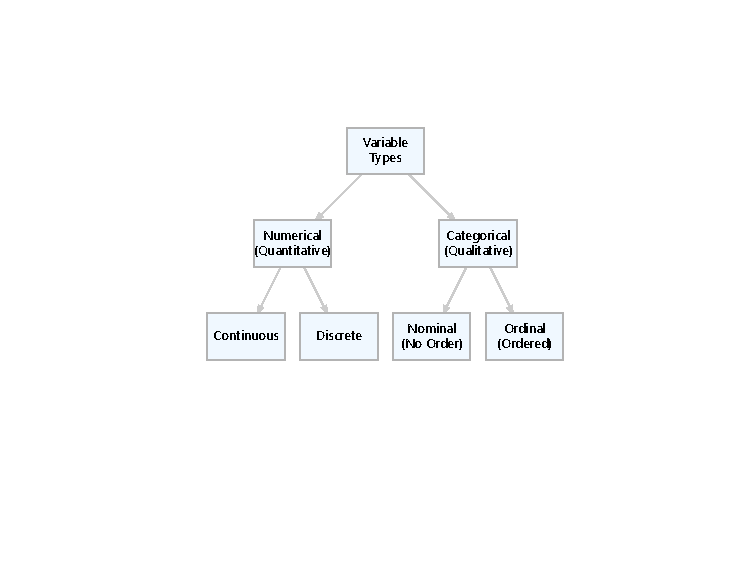
\includegraphics[width=1\textwidth, trim=90 95 90 50, clip]{Diagram-Variable-Types.pdf}
    %\caption{Cropped PDF Image}
    \label{fig:vartypes}
\end{figure}
\end{frame}

\begin{frame}{Example: Types of Variables}

Can you correctly identify the types of variables included in this dataset?
    \begin{itemize}
        \item \textbf{Sample Dataset:}
    \end{itemize}
        \begin{center}
                     \begin{tabular}{|c|c|c|c|c|c|c|}
            \hline
            \textbf{Respondent} & \textbf{Age} & \textbf{Income} & \textbf{$X_1$} & \textbf{$X_2$} & \textbf{State} & \textbf{Education} \\ \hline
            1 & 34 & 55000 & 1 & 7 & NY & High school \\ \hline
            2 & 29 & 60000 & 0 & 1 & NJ & Master’s \\  \hline
            3 & 45 & 70000 & 1 & 3 & MA & High school \\ \hline
            4 & 40 & 65000 & 0 & 4 & MA & High school \\ \hline
            5 & 38 & 62000 & 1 & 2 & NY & Bachelor’s \\  \hline
            \vdots & \vdots  & \vdots  & \vdots  & \vdots  & \vdots & \vdots   \\ \hline
        \end{tabular}
        \end{center}
\end{frame}

\transitionslide{Statistical Principles Involved in Research Studies}  %%%%%%%%%%%%%%%%%%%%%%%%%%%%%%%%%%%%%%%%%%%%%%%

\begin{frame}{Defining an Empiricist Research Question}
\textbf{Research Question:}
\begin{itemize}
    \item A question that seeks to explore observable and measurable phenomena.
    \item Must be testable through empirical data and direct observation.
    \item Aims to contribute to existing knowledge, test theories, or solve practical problems.
\end{itemize}
    \pause %%%%%%
\textbf{Example:}
\begin{itemize}
    \item \textbf{Poorly Defined:} ``Does exercise affect health?"
    \item \textbf{Well-Defined:} ``What is the impact of a 30-minute daily aerobic exercise regimen on the cardiovascular health markers (e.g., blood pressure, cholesterol levels) of adults aged 30-50 over six months?"
\end{itemize}

\end{frame}

\begin{frame}{Components of a Well Defined Research Question}
\begin{itemize}
    \item \textbf{Specificity:} Clearly defines variables and their relationships or differences, ensuring focus and clarity.
    \item \textbf{Operationalization:} Concepts are defined in measurable terms, facilitating precise data collection.
    \item \textbf{Feasibility:} The question is practical to investigate considering available resources, time, and ethical standards.
    \item \textbf{Relevance:} Addresses significant issues or gaps within the field.
    \item \textbf{Novelty:} Contributes new insights or perspectives to existing research.
\end{itemize}


\end{frame}




\begin{frame}{Example: Population and Research Question}
\textcolor{moonstoneblue}{\textbf{Research Question:}} What is the impact of a universal basic income (UBI) on economic stability and poverty reduction, specifically among low-income households?

\vspace{0.5cm}

\textcolor{moonstoneblue}{\textbf{Population of Interest:}} Low-income households across the entire country, with consideration of regional, demographic, and economic diversity.

\end{frame}


\begin{frame}{Associated and Independent Variables}
    \begin{itemize}
        \item \textbf{Associated Variables}: Variables that show some relationship with each other. The association can be \textbf{positive} (both increase and decrease together), \textbf{negative} (one increases while the other decreases), or \textbf{non-linear}.
        \item \textbf{Independent Variables}: Variables that are not associated and do not influence each other.
    \end{itemize}
\end{frame}

\begin{frame}{Example}
What is the association between the total number of community activities in a neighborhood and the level of social trust among its residents?
\vspace{7cm}
\end{frame}

\begin{frame}{Explanatory and Response Variables}
    \begin{itemize}
        \item \textbf{Explanatory Variable}: The variable suspected of affecting the other. Often considered the cause.    \pause  % <----> %
        \item \textbf{Response (Outcome) Variable}: The outcome or effect being measured.     \pause  % <----> %
        \item \textbf{Note}: \emph{Association between variables does not imply causality}, even if an explanatory-response relationship is identified.     \pause  % <----> %
    \end{itemize}

    \begin{figure}[h]
        \centering
        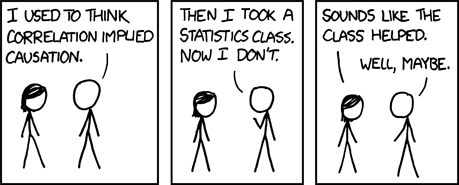
\includegraphics[width=0.5\linewidth]{correlation.png}
        \caption{Correlation (Source: \href{https://xkcd.com/552/}{XKCD})}
    \end{figure}
\end{frame}

\begin{frame}{Observational vs. Experimental Studies}
    \begin{tabular}{ l | p{0.33\textwidth} | p{0.33\textwidth} }
        \textbf{Aspect} & \textbf{Observational Study} & \textbf{Experimental Study} \\
        \hline
        \textbf{Definition} & Data collected without manipulating variables & Involves manipulating one or more variables \\ \pause  % <----> %
        & & \\
        \textbf{Purpose} & Identify associations between variables & Establish cause and effect relationships \\ \pause  % <----> %
                & & \\
        \textbf{Causation} & Cannot determine causality & Can determine causality with proper design \\
    \end{tabular}
\end{frame}

\begin{frame}{Confounding Variables and Statistical Bias}

    \begin{columns}[T] % Align columns at the top
        \column{0.48\textwidth}
            \begin{block}{Confounding Variables}
                \textbf{Definition:} Unaccounted variables that influence both the explanatory and response (outcome) variables. \pause %<---->%

                \vspace{0.2cm}

                \textbf{Impact:} Without controlling for confounders, researchers may \textbf{misattribute} the association between variables, incorrectly inferring a direct relationship. \pause %<---->%
            \end{block}

        \column{0.48\textwidth}
            \begin{block}{Statistical Bias}
                \textbf{Definition:} Systematic errors in data collection, analysis, interpretation, or review processes that can \textbf{distort} findings.
                \pause %<---->%
                \vspace{0.2cm}
                \textbf{Example:} \textit{Confounding Bias} is a distortion that alters the true association between an explanatory and an outcome variable due to a third factor that is independently associated with the exposure and the outcome (\href{https://catalogofbias.org/biases/confounding/}{Source}).
            \end{block}
    \end{columns}

\end{frame}




\begin{frame}{Example: Assessing the Impact of Math Tutoring}

    \textbf{Research Context:}

    A high school is implementing a new structured math tutoring program that provides students with an additional 2 hours of tutoring per week. Participation is voluntary. The goal is to determine whether this program positively affects students' performance in standardized math tests over the course of one academic year.

    \vspace{0.3cm}

    \textbf{Task:}

    Identify and describe \textbf{one variable} that could cause \textbf{confounding bias} when assessing the association between \textbf{participation in the math tutoring program (X)} and \textbf{standardized math test scores (Y)}.
\end{frame}

\begin{frame}{Experiments in Social Science}
    \textbf{Context:} \\
    Social science experiments help us understand cause-and-effect relationships by manipulating a specific variable (the \textit{treatment}) under controlled conditions. \pause %<---->%

    \vspace{0.3cm}

    \textbf{Experimental Treatment (Definition):}\\
    The specific intervention or condition applied exclusively to the \textbf{treatment group}. This allows researchers to measure its impact on the response (outcome) variable compared to the \textbf{control group} (untreated).

\end{frame}


\begin{frame}{Principles of Experimental Design}
    \begin{itemize}
        \item \textbf{Control}: Accounting for confounding factors to ensure observed effects are due to the treatment.
        \item \textbf{Randomization}: Randomly assigning subjects to treatment and control groups to eliminate selection bias. \pause %<---->%
        \item \textbf{Replication}: Repeating the experiment or using a sufficiently large sample to ensure the results are reliable.
        \item \textbf{Blocking}: Grouping subjects with similar characteristics to reduce variability and better isolate the treatment effect.
    \end{itemize}
\end{frame}

\begin{frame}{Blinding in Studies}
    \begin{itemize}
        \item \textbf{Single Blinding}: Participants are unaware of whether they are in the treatment or control group.
        \item \textbf{Double Blinding}: Both participants and experimenters are unaware of the group assignments. \pause %<---->%
        \item Blinding helps reduce bias, particularly the \href{https://catalogofbias.org/biases/performance-bias/}{Performance} and \href{https://dictionary.apa.org/experimenter-bias}{Experimenter} bias. \pause %<---->%
        \begin{itemize}
        \item E.g., in a clinical study, if participants in the control group systematically seek other treatments, there could be performance bias.
        \item Or, if researchers/clinicians treat participants differently depending on which group they are in, this could imply experimenter bias (see: \href{https://dictionary.apa.org/experimenter-effect}{Experimenter Effect}).
        \item  \textbf{Placebo Effect}: Change in participants' outcome variable due to their belief in the treatment rather than the treatment itself.
        \end{itemize}
    \end{itemize}
\end{frame}

\transitionslide{Sampling: Basic Principles}  %%%%%%%%%%%%%%%%%%%%%%%%%%%%%%%%%%%%%%%%%%%%%%%

\begin{frame}{Sampling Methods and Sampling Bias}

    \textbf{Sampling Method (Definition):} \\
    A \href{https://dictionary.apa.org/sampling}{sampling} method refers to the process used to select individuals or observations from a population to be included in a sample.
    \newline

    \textbf{Sampling Bias (General):}
    \begin{itemize}
        \item
        \href{https://dictionary.apa.org/sampling-bias}{Sampling bias} occurs when the process of selecting a sample \textbf{skews the results}, making some members of the population systematically more (or less) likely to be included than others.
    \end{itemize}

\end{frame}

\begin{frame}{Sampling Methods and Sampling Bias}

    \textbf{Types of Sampling Bias:}
    \begin{itemize}
        \item \textbf{Non-response Bias:}
        Arises when individuals selected for the sample do not respond or are unwilling to participate, and those non-responders \textbf{differ in important ways} from those who do respond. \pause %<---->%

        \item \textbf{Self-Selection Bias:}
        Occurs when participation in a survey, study, or experiment is \textbf{voluntary}, allowing individuals to decide on their own whether to be included. As a result, those who opt-in may \textbf{systematically differ} from those who do not, leading to a non-representative sample. \pause

        \item \textbf{Coverage Bias:}
        Happens when some members of the population are inadequately represented in the sample due to limitations in the \textbf{sampling frame}. This occurs when certain groups have \textbf{no chance} or a \textbf{lower chance} of being included, leading to a distorted view of the population.
        \begin{itemize}
            \item \textbf{Sampling Frame:} The list or method used to identify and select individuals from the population for inclusion in the sample.
        \end{itemize}
    \end{itemize}

\end{frame}





\begin{frame}{Probabilistic Sampling}
    \begin{itemize}
        \item \textbf{Probabilistic Sampling (def.):} A method where each member of the population has a known, non-zero chance of being selected in the sample. This approach ensures that the sample is more representative of the population.
        \begin{itemize}
            \item \textbf{Examples:} Simple random sampling, stratified sampling, cluster sampling.
        \end{itemize}

        \item \textbf{Advantages:} Reduces sampling bias, allows for generalization to the population, and facilitates the use of statistical inference.
    \end{itemize}

\end{frame}

\begin{frame}{Sampling Techniques}
    \begin{itemize}
        \item \textbf{Simple Random Sampling}: Every subject has an equal probability of being selected. \pause %<---->%
        \item \textbf{Stratified Sampling}: Population is divided into strata; a random sample is drawn from each stratum. \pause %<---->%
        \item \textbf{Cluster Sampling}: Population is divided into clusters (i.e., naturally forming groups that are diverse within and similar between); a random sample of clusters is selected, and all subjects within those clusters are studied. \pause %<---->%
        \item \textbf{Multistage Sampling}: Corresponds to taking samples in stages using smaller and smaller sampling units at each stage.
        \begin{itemize}
            \item For example, clusters are chosen randomly, and then a random sample from within each cluster is selected.
        \end{itemize}
    \end{itemize}
\end{frame}

\begin{frame}{Stratified vs.\ Cluster Sampling}

{ \small
\begin{columns}[T]
   \column{0.47\textwidth}
    \textbf{Stratified Sampling}
    \begin{itemize}
        \item \textbf{Objective:} Ensure representation across distinct subgroups
        \item \textbf{When to Use:}
        \begin{itemize}
            \item Population is heterogeneous and can be divided into meaningful strata
            \item Detailed analysis is required within each subgroup
            \item High precision in estimates across strata
        \end{itemize} \pause %<---->%
        \item \textbf{Example:} Survey different income brackets to study economic disparities  \pause %<---->%
    \end{itemize}

    \column{0.47\textwidth}
    \textbf{Cluster Sampling}
    \begin{itemize}
        \item \textbf{Objective:} Reduce cost and logistical complexity for large, dispersed populations
        \item \textbf{When to Use:}
        \begin{itemize}
            \item Population naturally forms clusters
            \item Easier to collect data from entire clusters than from scattered individuals
            \item Ideally, each cluster is diverse internally (a “mini-population”)
        \end{itemize} \pause %<---->%
        \item \textbf{Example:} Conduct a health survey by sampling entire schools as clusters
    \end{itemize}
\end{columns}
}
\end{frame}


\begin{frame}{Convenience (Non-probabilistic) Sampling}

    \begin{itemize}
        \item \textbf{Convenience (Non-probabilistic) Sampling (def.):} Individuals who are easiest to reach or most accessible are chosen for the sample, rather than randomly or systematically selected.
        \item \textbf{Potential Issues:}
        \begin{itemize}
            \item \textbf{Bias:} May result in a sample that is not representative of the population. Findings may not be applicable to the broader population due to the non-random nature of sample selection.
            \item \textbf{Examples:} Surveying people in a mall or using participants from a single location or organization.
        \end{itemize}
    \end{itemize}
\end{frame}

\begin{frame}{Representativeness of a Sample}
    \textbf{Definition:}
    A sample is \textbf{representative} if its key characteristics (e.g., demographics, behaviors) closely match those of the overall population, allowing for valid generalizations.
    \newline  \pause %<---->%

    \textbf{Discussion:}
    \begin{itemize}
        \item \emph{Survey Vendors}:
        Many commercial survey vendors sell \textbf{representative samples} based on a few demographic features
        \textcolor{red}{ but not true probabilistic samples}, meaning results may still be affected by sampling bias.
        \begin{itemize}
            \item The most common form of representative sample is \href{https://dictionary.apa.org/quota-sampling}{quota sampling}.
        \end{itemize}  \pause %<---->%
        \item Even a probabilistic sample can be \textbf{non-representative} if it is too small or improperly stratified.
    \end{itemize}

\end{frame}



\transitionslide{Terms and Concepts Covered} %%%%%%%%%%%%%%%%%%%%%

% Final slide listing all terms covered in the lecture
\begin{frame}{Terms and Concepts Covered in this Lecture}
  \addtocounter{framenumber}{-1}
\footnotesize
    \begin{columns}
        \begin{column}{0.5\textwidth}
            \begin{itemize}
                \item Statistics
                \item Population
                \item Sample
                \item Estimator
                \item Statistical Inference
                \item Dataset, Observations, \& Variables
                \item Categorical/Continuous Variables
                \item Response/Explanatory Variable
                \item Observational/Experimental Study
                \item Confounding Variables
                \item Bias
                \item Sampling Techniques
            \end{itemize}
        \end{column}
        \begin{column}{0.5\textwidth}
            \begin{itemize}

                \item Voluntary Response
                \item Simple Random Sampling / Stratified / Cluster / Multistage Sampling
                \item Research Question
                \item Population of Interest
                \item Associated/Independent Variables
                \item Blinding
                \item Control
                \item Randomization
                \item Replication
                \item Blocking
                \item Sampling Bias
                \item Convenience Sampling Bias
            \end{itemize}
        \end{column}
    \end{columns}
\end{frame}

\end{document}

## 1. **Coverage Bias (Undercoverage)**
- **Definition:** Occurs when the sampling frame **systematically excludes** certain segments of the population.
- **Example:** Conducting a telephone survey but only calling landlines could underrepresent younger or more mobile individuals who rely exclusively on cell phones.
- **Result:** The sample fails to represent the population accurately because some groups have **no chance** or a disproportionately lower chance of being included.

---

## 2. **Convenience Sampling Bias**
- **Definition:** Arises when a sample is selected primarily because it is **easily accessible**, rather than through a probability-based method.
- **Example:** Surveying only your classmates or people walking past a single location at a specific time.
- **Result:** The sample is unlikely to represent the broader population, as it overrepresents individuals who are readily available in that particular setting.

    \begin{alertblock}{Why It Matters}
        Both confounding variables and bias can **compromise** the validity of research, leading to incorrect conclusions. Understanding and mitigating them is essential for credible studies.
    \end{alertblock}

In general, **survey weights** reflect the inverse of an individual’s probability of being selected into the sample. For a (typical) two-stage cluster design:

1. **Stage 1: Select Clusters**
   Suppose there are \( M \) total clusters in the population, and you randomly select \( m \) of them. If each cluster is equally likely to be chosen, then the probability that a specific cluster \(i\) is selected is
   \[
   p_i = \frac{m}{M}.
   \]

2. **Stage 2: Select Individuals Within Each Selected Cluster**
   Let cluster \(i\) contain \( N_i \) individuals, and you draw a sample of \( n_i \) individuals. If this selection is simple random sampling within cluster \(i\), then each individual in that cluster has probability
   \[
   q_i = \frac{n_i}{N_i}
   \]
   of being chosen (given that cluster \(i\) was selected in the first place).

---

### Computing the Weights

- **Overall selection probability** for an individual \(j\) in cluster \(i\) is
  \[
  \text{Prob}(\text{select } j) \;=\; p_i \times q_i.
  \]

- **Survey weight** for that individual is the inverse of the selection probability:
  \[
  w_{ij} = \frac{1}{p_i \times q_i}.
  \]

### Common Special Case

If each cluster has the same number of individuals (say \(N\) each) and you select the same sample size \(n\) per cluster, and all clusters are equally likely to be chosen, then the weight simplifies to:
\[
w_{ij} \;=\; \frac{M}{m} \;\times\; \frac{N}{n}.
\]

---

In practice:
- If different clusters have different probabilities of selection, you must use each cluster’s actual selection probability \(p_i\).
- Similarly, if different numbers of individuals are sampled from each cluster, use each cluster’s actual within-cluster sampling probability \(q_i\).
- Finally, many surveys refine these “base weights” with additional adjustments (e.g., for non-response or post-stratification), but the fundamental step always starts with **inverse of selection probability**.
